\documentclass[10pt,twocolumn,letterpaper]{article}

\usepackage{iccv}
\usepackage{times}
\usepackage{epsfig}
\usepackage{graphicx}
\usepackage{color}
\usepackage{caption}
\usepackage{amsmath}
\usepackage{amssymb}
\usepackage{bm}
\usepackage{booktabs}
\usepackage{lib}
\usepackage{algorithm}
\usepackage{algpseudocode}

\usepackage[pagebackref=true,breaklinks=true,letterpaper=true,colorlinks,bookmarks=false]{hyperref}

\iccvfinalcopy % *** Uncomment this line for the final submission

\def\iccvPaperID{1772} % *** Enter the ICCV Paper ID here
\def\httilde{\mbox{\tt\raisebox{-.5ex}{\symbol{126}}}}

% Pages are numbered in submission mode, and unnumbered in camera-ready
\ificcvfinal\pagestyle{empty}\fi
\begin{document}

%%%%%%%%% TITLE
\title{Amodal Completion and Size Constancy in Natural Scenes:\\Supplementary Material}
%\title{Object Size from a Single Image}

\author{Abhishek Kar, Shubham Tulsiani, Jo\~{a}o Carreira and Jitendra Malik\\
University of California, Berkeley - Berkeley, CA 94720\\
{\tt\small \{akar,shubhtuls,carreira,malik\}@eecs.berkeley.edu}}

\maketitle
%\thispagestyle{empty}
\section{Additional Results}
We present more qualitative results of our amodal completion and size inference algorithm in this document. All the results are obtained by using our class agnostic amodal completion network on ground truth boxes in the PASCAL VOC \textit{val} set and estimating sizes using our size inference algorithm on these amodal boxes. Each row shows the original image, the ground truth box annotations in PASCAL and finally the amodal boxes along with inferred sizes and the horizon (shown by the horizontal red line). 

We also show the distribution of camera heights inferred using our algorithm in \figref{heightDistr} and the focal lengths used for training our CNN focal length predictor in \figref{fovDistr}.

\begin{figure}[b]
    \centering
    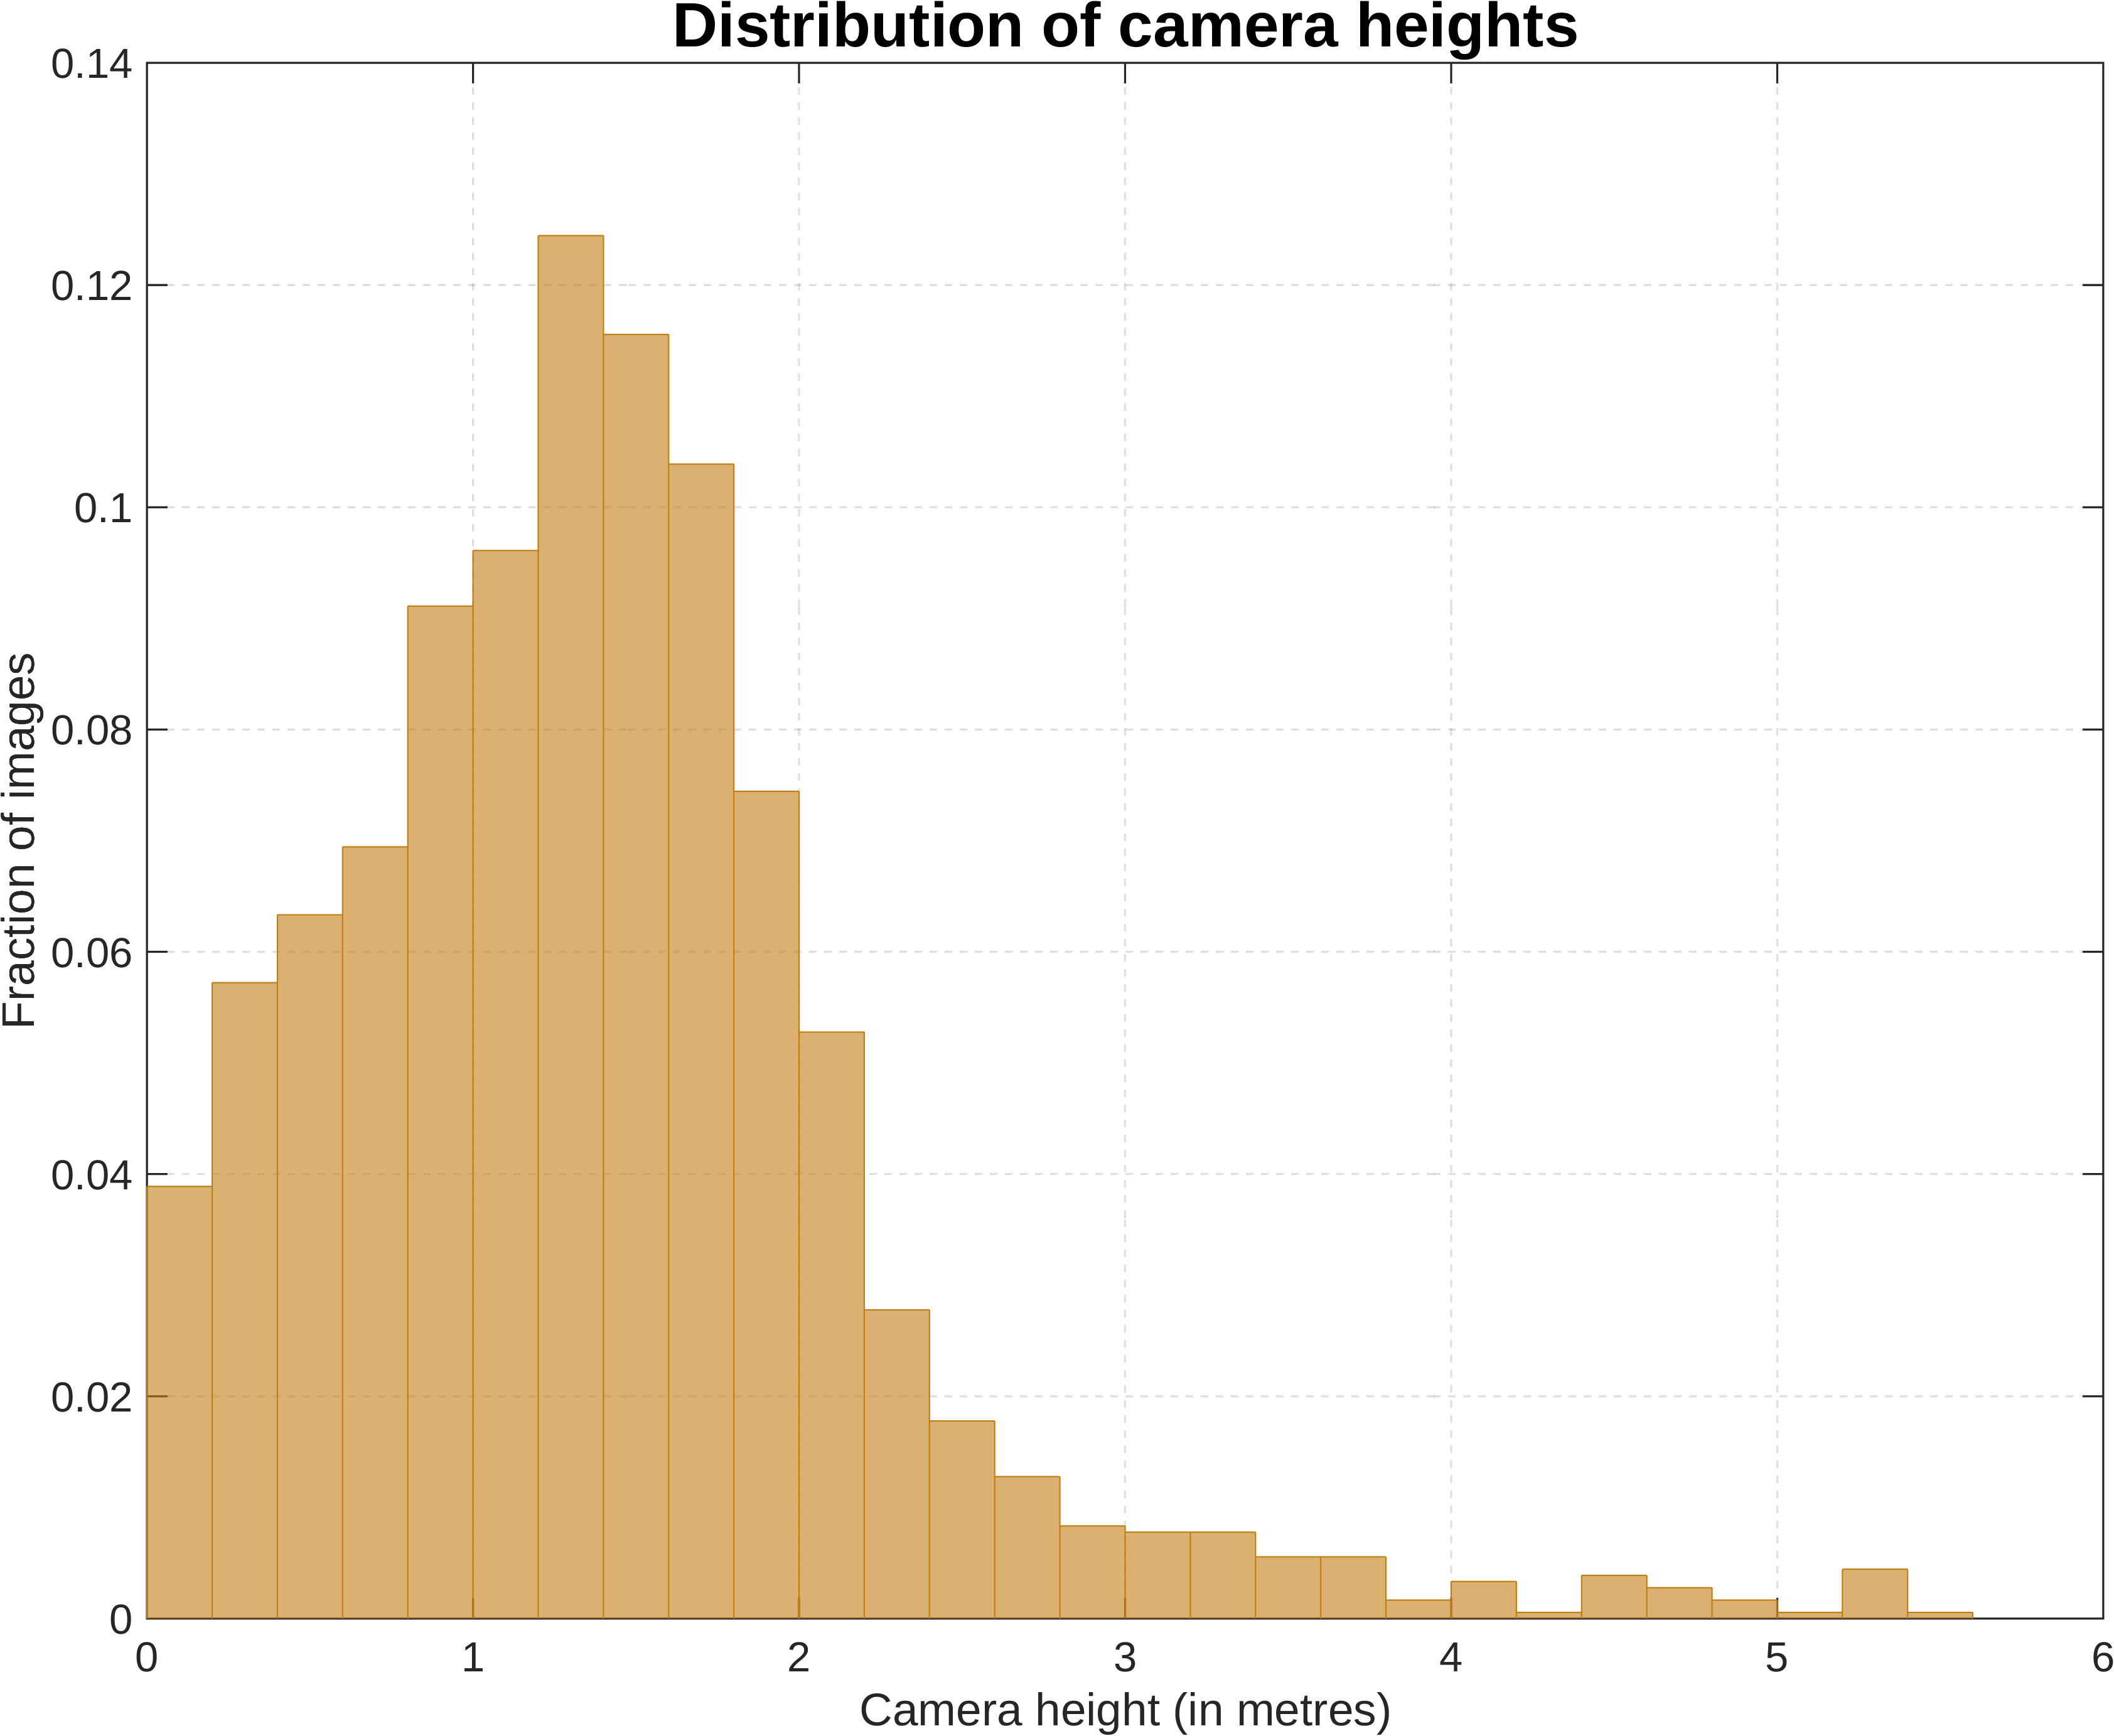
\includegraphics[width=0.48\textwidth]{figures/amodal/heights_pred_choc.png}
    \caption{\figlabel{heightDistr} Distribution of camera heights as inferred on PASCAL VOC. It can be seen that the distribution is peaked around the height at which humans normally take pictures (1.4m) with a long tail.}
\end{figure}
\begin{figure}[t!]
    \centering
    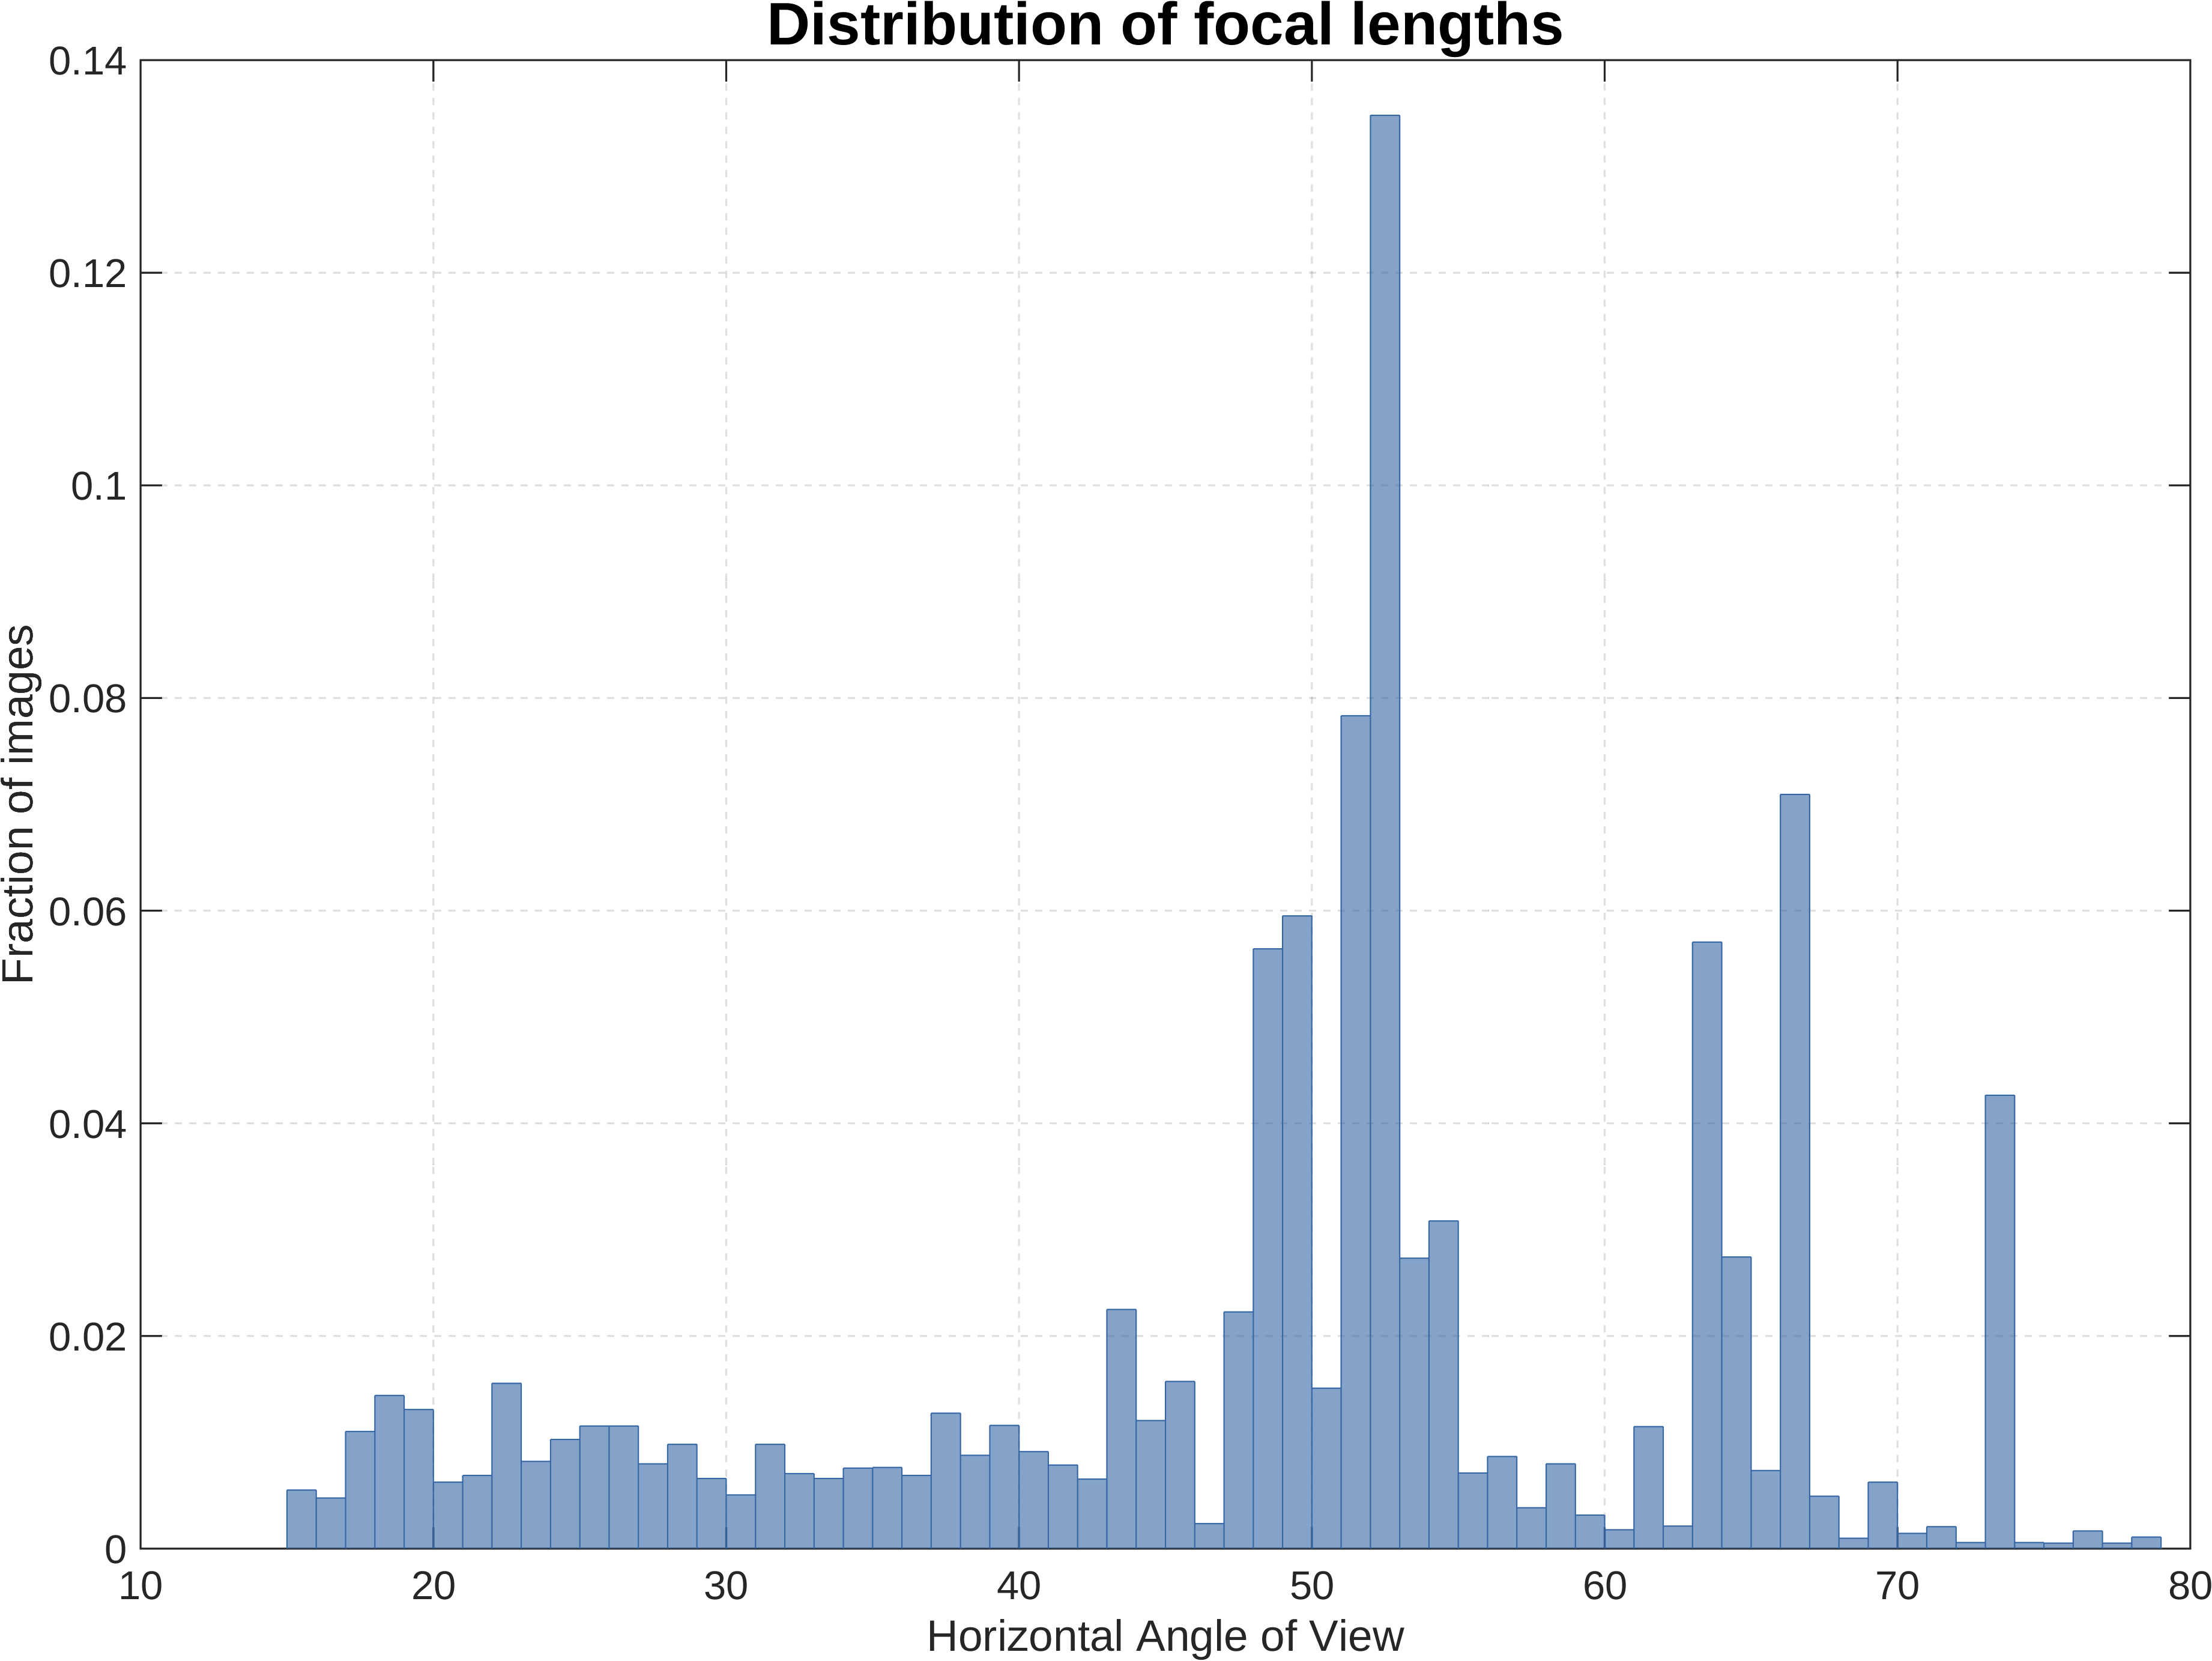
\includegraphics[width=0.48\textwidth]{figures/amodal/fov.png}
    \caption{\figlabel{fovDistr} Distribution of camera focal lengths in the Places dataset shown as horizontal angle of view. The peaks in the distribution correspond to canonical focal lengths in popular wide angle and telephoto lenses. It can be seen that the images cover the full spectrum from wide angle views of scenes (corresponding to the right end of the plot) to close-ups (left end of the histogram). Interestingly, the largest peak in the distribution is close to the field of view of iPhones.}
\end{figure}
\begin{figure*}
\centering\includegraphics[height=0.2\textwidth]{figures/amodal/supplementary/2008_006467_im.png}
\includegraphics[height=0.2\textwidth]{figures/amodal/supplementary/2008_006467_gt.png}
\includegraphics[height=0.2\textwidth]{figures/amodal/supplementary/2008_006467_amod.png} \\ 
\includegraphics[height=0.2\textwidth]{figures/amodal/supplementary/2009_004974_im.png}
\includegraphics[height=0.2\textwidth]{figures/amodal/supplementary/2009_004974_gt.png}
\includegraphics[height=0.2\textwidth]{figures/amodal/supplementary/2009_004974_amod.png} \\ 
\includegraphics[height=0.2\textwidth]{figures/amodal/supplementary/2008_006382_im.png}
\includegraphics[height=0.2\textwidth]{figures/amodal/supplementary/2008_006382_gt.png}
\includegraphics[height=0.2\textwidth]{figures/amodal/supplementary/2008_006382_amod.png} \\ 
\includegraphics[height=0.2\textwidth]{figures/amodal/supplementary/2009_002398_im.png}
\includegraphics[height=0.2\textwidth]{figures/amodal/supplementary/2009_002398_gt.png}
\includegraphics[height=0.2\textwidth]{figures/amodal/supplementary/2009_002398_amod.png} \\ 
\includegraphics[height=0.2\textwidth]{figures/amodal/supplementary/2008_004613_im.png}
\includegraphics[height=0.2\textwidth]{figures/amodal/supplementary/2008_004613_gt.png}
\includegraphics[height=0.2\textwidth]{figures/amodal/supplementary/2008_004613_amod.png} \\ 
\includegraphics[height=0.2\textwidth]{figures/amodal/supplementary/2008_003132_im.png}
\includegraphics[height=0.2\textwidth]{figures/amodal/supplementary/2008_003132_gt.png}
\includegraphics[height=0.2\textwidth]{figures/amodal/supplementary/2008_003132_amod.png} \\ 
\end{figure*}
\begin{figure*}
\centering\includegraphics[height=0.2\textwidth]{figures/amodal/supplementary/2009_001754_im.png}
\includegraphics[height=0.2\textwidth]{figures/amodal/supplementary/2009_001754_gt.png}
\includegraphics[height=0.2\textwidth]{figures/amodal/supplementary/2009_001754_amod.png} \\ 
\includegraphics[height=0.2\textwidth]{figures/amodal/supplementary/2009_001635_im.png}
\includegraphics[height=0.2\textwidth]{figures/amodal/supplementary/2009_001635_gt.png}
\includegraphics[height=0.2\textwidth]{figures/amodal/supplementary/2009_001635_amod.png} \\ 
\includegraphics[height=0.2\textwidth]{figures/amodal/supplementary/2009_003973_im.png}
\includegraphics[height=0.2\textwidth]{figures/amodal/supplementary/2009_003973_gt.png}
\includegraphics[height=0.2\textwidth]{figures/amodal/supplementary/2009_003973_amod.png} \\ 
\includegraphics[height=0.2\textwidth]{figures/amodal/supplementary/2010_004877_im.png}
\includegraphics[height=0.2\textwidth]{figures/amodal/supplementary/2010_004877_gt.png}
\includegraphics[height=0.2\textwidth]{figures/amodal/supplementary/2010_004877_amod.png} \\ 
\includegraphics[height=0.2\textwidth]{figures/amodal/supplementary/2008_006010_im.png}
\includegraphics[height=0.2\textwidth]{figures/amodal/supplementary/2008_006010_gt.png}
\includegraphics[height=0.2\textwidth]{figures/amodal/supplementary/2008_006010_amod.png} \\ 
\includegraphics[height=0.2\textwidth]{figures/amodal/supplementary/2011_001223_im.png}
\includegraphics[height=0.2\textwidth]{figures/amodal/supplementary/2011_001223_gt.png}
\includegraphics[height=0.2\textwidth]{figures/amodal/supplementary/2011_001223_amod.png} \\ 
\end{figure*}
\begin{figure*}
\centering\includegraphics[height=0.2\textwidth]{figures/amodal/supplementary/2010_004469_im.png}
\includegraphics[height=0.2\textwidth]{figures/amodal/supplementary/2010_004469_gt.png}
\includegraphics[height=0.2\textwidth]{figures/amodal/supplementary/2010_004469_amod.png} \\ 
\includegraphics[height=0.2\textwidth]{figures/amodal/supplementary/2008_005032_im.png}
\includegraphics[height=0.2\textwidth]{figures/amodal/supplementary/2008_005032_gt.png}
\includegraphics[height=0.2\textwidth]{figures/amodal/supplementary/2008_005032_amod.png} \\ 
\includegraphics[height=0.2\textwidth]{figures/amodal/supplementary/2010_000262_im.png}
\includegraphics[height=0.2\textwidth]{figures/amodal/supplementary/2010_000262_gt.png}
\includegraphics[height=0.2\textwidth]{figures/amodal/supplementary/2010_000262_amod.png} \\ 
\includegraphics[height=0.2\textwidth]{figures/amodal/supplementary/2010_004785_im.png}
\includegraphics[height=0.2\textwidth]{figures/amodal/supplementary/2010_004785_gt.png}
\includegraphics[height=0.2\textwidth]{figures/amodal/supplementary/2010_004785_amod.png} \\ 
\includegraphics[height=0.2\textwidth]{figures/amodal/supplementary/2009_001326_im.png}
\includegraphics[height=0.2\textwidth]{figures/amodal/supplementary/2009_001326_gt.png}
\includegraphics[height=0.2\textwidth]{figures/amodal/supplementary/2009_001326_amod.png} \\ 
\includegraphics[height=0.2\textwidth]{figures/amodal/supplementary/2008_007716_im.png}
\includegraphics[height=0.2\textwidth]{figures/amodal/supplementary/2008_007716_gt.png}
\includegraphics[height=0.2\textwidth]{figures/amodal/supplementary/2008_007716_amod.png} \\ 
\end{figure*}
\begin{figure*}
\centering\includegraphics[height=0.15\textwidth]{figures/amodal/supplementary/2011_000518_im.png}
\includegraphics[height=0.15\textwidth]{figures/amodal/supplementary/2011_000518_gt.png}
\includegraphics[height=0.15\textwidth]{figures/amodal/supplementary/2011_000518_amod.png} \\ 
\includegraphics[height=0.2\textwidth]{figures/amodal/supplementary/2008_003514_im.png}
\includegraphics[height=0.2\textwidth]{figures/amodal/supplementary/2008_003514_gt.png}
\includegraphics[height=0.2\textwidth]{figures/amodal/supplementary/2008_003514_amod.png} \\ 
\includegraphics[height=0.2\textwidth]{figures/amodal/supplementary/2011_002093_im.png}
\includegraphics[height=0.2\textwidth]{figures/amodal/supplementary/2011_002093_gt.png}
\includegraphics[height=0.2\textwidth]{figures/amodal/supplementary/2011_002093_amod.png} \\ 
\includegraphics[height=0.2\textwidth]{figures/amodal/supplementary/2010_004533_im.png}
\includegraphics[height=0.2\textwidth]{figures/amodal/supplementary/2010_004533_gt.png}
\includegraphics[height=0.2\textwidth]{figures/amodal/supplementary/2010_004533_amod.png} \\ 
\includegraphics[height=0.2\textwidth]{figures/amodal/supplementary/2009_001184_im.png}
\includegraphics[height=0.2\textwidth]{figures/amodal/supplementary/2009_001184_gt.png}
\includegraphics[height=0.2\textwidth]{figures/amodal/supplementary/2009_001184_amod.png} \\ 
\includegraphics[height=0.2\textwidth]{figures/amodal/supplementary/2009_002570_im.png}
\includegraphics[height=0.2\textwidth]{figures/amodal/supplementary/2009_002570_gt.png}
\includegraphics[height=0.2\textwidth]{figures/amodal/supplementary/2009_002570_amod.png} \\ 
\end{figure*}
\begin{figure*}
\centering\includegraphics[height=0.2\textwidth]{figures/amodal/supplementary/2011_001870_im.png}
\includegraphics[height=0.2\textwidth]{figures/amodal/supplementary/2011_001870_gt.png}
\includegraphics[height=0.2\textwidth]{figures/amodal/supplementary/2011_001870_amod.png} \\ 
\includegraphics[height=0.2\textwidth]{figures/amodal/supplementary/2011_001951_im.png}
\includegraphics[height=0.2\textwidth]{figures/amodal/supplementary/2011_001951_gt.png}
\includegraphics[height=0.2\textwidth]{figures/amodal/supplementary/2011_001951_amod.png} \\ 
\includegraphics[height=0.2\textwidth]{figures/amodal/supplementary/2009_002055_im.png}
\includegraphics[height=0.2\textwidth]{figures/amodal/supplementary/2009_002055_gt.png}
\includegraphics[height=0.2\textwidth]{figures/amodal/supplementary/2009_002055_amod.png} \\ 
\includegraphics[height=0.2\textwidth]{figures/amodal/supplementary/2008_000418_im.png}
\includegraphics[height=0.2\textwidth]{figures/amodal/supplementary/2008_000418_gt.png}
\includegraphics[height=0.2\textwidth]{figures/amodal/supplementary/2008_000418_amod.png} \\ 
\includegraphics[height=0.2\textwidth]{figures/amodal/supplementary/2009_005171_im.png}
\includegraphics[height=0.2\textwidth]{figures/amodal/supplementary/2009_005171_gt.png}
\includegraphics[height=0.2\textwidth]{figures/amodal/supplementary/2009_005171_amod.png} \\ 
\includegraphics[height=0.2\textwidth]{figures/amodal/supplementary/2009_005203_im.png}
\includegraphics[height=0.2\textwidth]{figures/amodal/supplementary/2009_005203_gt.png}
\includegraphics[height=0.2\textwidth]{figures/amodal/supplementary/2009_005203_amod.png} \\ 
\end{figure*}
\begin{figure*}
\centering\includegraphics[height=0.2\textwidth]{figures/amodal/supplementary/2009_004303_im.png}
\includegraphics[height=0.2\textwidth]{figures/amodal/supplementary/2009_004303_gt.png}
\includegraphics[height=0.2\textwidth]{figures/amodal/supplementary/2009_004303_amod.png} \\ 
\includegraphics[height=0.2\textwidth]{figures/amodal/supplementary/2009_002346_im.png}
\includegraphics[height=0.2\textwidth]{figures/amodal/supplementary/2009_002346_gt.png}
\includegraphics[height=0.2\textwidth]{figures/amodal/supplementary/2009_002346_amod.png} \\ 
\includegraphics[height=0.2\textwidth]{figures/amodal/supplementary/2008_003022_im.png}
\includegraphics[height=0.2\textwidth]{figures/amodal/supplementary/2008_003022_gt.png}
\includegraphics[height=0.2\textwidth]{figures/amodal/supplementary/2008_003022_amod.png} \\ 
\includegraphics[height=0.2\textwidth]{figures/amodal/supplementary/2010_001851_im.png}
\includegraphics[height=0.2\textwidth]{figures/amodal/supplementary/2010_001851_gt.png}
\includegraphics[height=0.2\textwidth]{figures/amodal/supplementary/2010_001851_amod.png} \\ 
\includegraphics[height=0.2\textwidth]{figures/amodal/supplementary/2008_006547_im.png}
\includegraphics[height=0.2\textwidth]{figures/amodal/supplementary/2008_006547_gt.png}
\includegraphics[height=0.2\textwidth]{figures/amodal/supplementary/2008_006547_amod.png} \\ 
\includegraphics[height=0.17\textwidth]{figures/amodal/supplementary/2009_002566_im.png}
\includegraphics[height=0.17\textwidth]{figures/amodal/supplementary/2009_002566_gt.png}
\includegraphics[height=0.17\textwidth]{figures/amodal/supplementary/2009_002566_amod.png} \\ 
\end{figure*}

\end{document}
